	\documentclass[tikz,border = 10pt]{standalone}
 
%tikzpicture
\usepackage{tikz}
\usepackage{scalerel}
\usepackage{pict2e}
\usepackage{tkz-euclide}
\usetikzlibrary{calc}
\usetikzlibrary{patterns,arrows.meta}
\usetikzlibrary{shadows}
\usetikzlibrary{external}


\usepackage{stix,graphicx}
 
 
\begin{document}
 \newcommand{\centerofmass}{{\ooalign{$\circleurquadblack$\cr\rotatebox[origin=c]{180}{$\circleurquadblack$}}}}

 
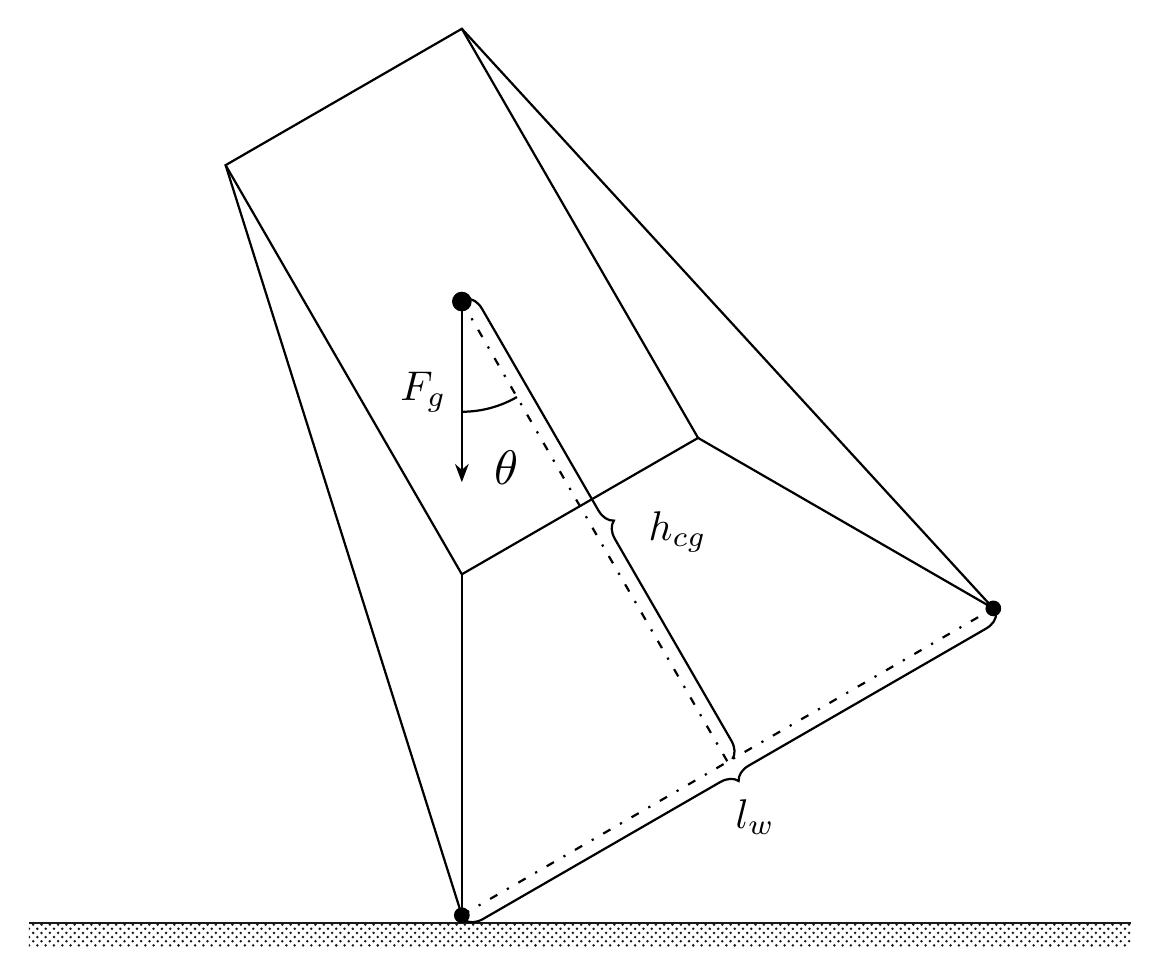
\begin{tikzpicture} [thick]
 



\draw [black!80!gray] (-10,-0.1) -- (4,-0.1);
\fill [pattern = crosshatch dots,
    pattern color = black!80!gray] (-10,-0.1) rectangle (4,-.4);
    


\coordinate (A) at (-4.5,4.3301268);
\coordinate (B) at (-7.5,9.5262792);
\coordinate (C) at (-4.5,11.2583304);
\coordinate (D)   at (-1.5,6.062178);
\coordinate(E) at (-4.5,4.3301268);
\coordinate(F) at (-4.5,7.7942286);
\coordinate(G) at (-1.1250000,1.9485572);

\draw (A) -- (B) -- (C) -- (D) -- (A);
\draw (A) -- (-4.5,0);
\draw (B) -- (-4.5,0);
\fill (-4.5,0) circle [radius = 0.1];

\draw (D) -- (2.25,3.8971146);
\draw (C) -- (2.25,3.8971146);
\fill (2.25,3.8971146) circle [radius = 0.1];

\draw[decorate,decoration={brace,raise=2pt,amplitude=6pt,mirror}] (-4.5,0)  -- (2.25,3.8971146) node[yshift = -20,xshift = 10,scale = 1.5,midway]{$l_w$};

\draw[decorate,decoration={brace,raise=2pt,amplitude=6pt}] (F) -- (G) node[scale = 1.5,midway,xshift = 20] {$h_{cg}$};

\draw[-Stealth] (F) -- (-4.5,5.5) node [midway,left,scale =1.5] {$F_g$};


%%https://www.ubuntu-user.com/Magazine/Archive/2014/22/Creating-vector-graphics-with-LaTeX-and-TikZ/%28offset%29/2

\draw[loosely dashdotted] (F)--(G);

\draw[loosely dashdotted] (-4.5,0)--(2.25,3.8971146);




\tkzMarkAngle[mark = none, size = 1.4cm](E,F,G);
\tkzLabelAngle[pos = 1.25,scale = 1.75](E,F,G){$\theta$};


\fill (F) circle [radius = 0.125];

\end{tikzpicture}
 
 
 
\end{document}